\documentclass [10pt]{article}
\usepackage{subfigure,graphics,graphicx,color,cite,multirow,rotating,epsfig}
%\usepackage[linesnumbered,figure,commentsnumbered]{algorithm2e}
%\usepackage[small]{titlesec}
\usepackage{microtype,caption}
\usepackage{xspace}
\usepackage{url}
\usepackage[T1]{fontenc}
\usepackage{helvet}
\renewcommand*\familydefault{\sfdefault} 
\usepackage{outlines}
\usepackage{setspace}
\usepackage{enumitem}


%\usepackage[dvips]{color}
%\usepackage[xdvi]{graphicx}

% \usepackage{oudraft}

\usepackage{color}
%\usepackage[pdfborder={0 0 0}]{hyperref}

% To make the FIXMEs go away, comment out this line...
\newcommand{\fixme}[1]{{\bf\textcolor{red}{[#1]}}}
% ...and uncomment this one.
%\newcommand{\fixme}[1]{}
\newcommand\eat[1]{}

% Have a margin of one inch on each side
\oddsidemargin  0.0in
\evensidemargin 0.0in
\topmargin      0.0in
\headheight     0.0in
\headsep        0.0in
\textheight     9in
\textwidth      6.5in
\topskip        0.0in
\footskip       0.15in
\marginparwidth 0in
\marginparsep   0in

% peanut gallery comments
%
%
% NOTE: Comment *in* the line below if you want a draft with no red comments.
% NOTE: Doing so may replace some of the red comments with 
%       extra spaces or newlines.
%\def\noeditingmarks{}
%
\newcommand{\textred}[1]{\textcolor{red}{#1}}
\ifx\noeditingmarks\undefined
   \newcommand{\pgwrapper}[2]{\textred{#1: #2}}
\else
   \newcommand{\pgwrapper}[2]{}
\fi
\newcommand{\note}[1]{\pgwrapper{NOTE}{#1}}
\newcommand{\sjs}[1]{\pgwrapper{SJS}{#1}}
\newcommand{\tk}[1]{\pgwrapper{TK}{#1}}

% end peanut gallery comments

\newenvironment{Itemize}%
{\begin{itemize}%
\setlength{\itemsep}{0pt}%
\setlength{\topsep}{0pt}%
\setlength{\partopsep}{0pt}%
\setlength{\parskip}{8pt}}%
{\end{itemize}}
\setlength{\leftmargini}{9pt}%

\newenvironment{Enumerate}%
{\begin{enumerate}%
\setlength{\itemsep}{0pt}%
\setlength{\topsep}{0pt}%
\setlength{\partopsep}{0pt}%
\setlength{\parskip}{0pt}}%
{\end{enumerate}}
\setlength{\leftmargini}{9pt}%

\newcommand{\name}{{FII}\xspace}
\newcommand{\dspace}{\baselineskip 25 pt}       % double spacing command
\newcommand{\sspace}{\baselineskip 14 pt}       % single spacing command
\newcommand{\xref}[1]{\S~\ref{#1}}
\newcommand{\pxref}[1]{(\xref{#1})}
\newcommand{\eg}{{\it e.g., }}
\newcommand{\ie}{{\it i.e., }}
\newcommand{\bi}{\begin{Itemize}}
\newcommand{\ei}{\end{Itemize}}


\hyphenation{trace-route}

\newtheorem{theorem}{Theorem}
%\newcommand{\bi}{\begin{itemize*}}
%\newcommand{\ei}{\end{itemize*}}
\newcommand{\im}{\item}
\begin{document}
\pagestyle{empty}



\newpage


\begin{center}
{\Large {\bf Secure, Real-Time Decisions on Live Data}}
\end{center}

{%\large
\setstretch{1.17}
{\bf Intellectual Merit:}  In just ten short years, the development of the open source big data processing systems, such as Hadoop, Hive, Storm, and more recently Spark~\cite{spark} and Kafka have fundamentally transformed daily practices in business and science. These systems have enabled the creation of new business models (e.g., Facebook, Twitter), the disruption of existing industries (e.g, Amazon, Uber, and Airbnb), and rapid progress in scientific research (cancer genomics, astronomy, social sciences). 
%\jmh{you'll need citations for the research to make NSF happy.  is there a Science or Nature paper that surveys big data in science?  i did a little search for Hadoop in Science and Nature on Google scholar and got a few hits like this: http://www.nature.com/nature/journal/v498/n7453/full/498255a.html}

Today, we are finding ourselves at another inflection point in big data processing that will define the next decade. This change is driven by three trends:

\begin{itemize}[noitemsep,topsep=0pt,parsep=0pt,partopsep=0pt]
\item Our world is becoming ever more connected, with sensors being now embedded in buildings, appliances, engines, wearable devices, clothes and more. With many of these sensors being connected to the Internet we can now sense the world around us in real-time at unprecedented scale.
\item With the advent of drones and self-driving cars we are now able not only to observe, but to make automated decisions that impact the physical world.
\item The success of applications such as high-frequency trading and ad bidding have demonstrated the tremendous value of making real-time decisions on live data.
\end{itemize}

These trends give us a glimpse of a future in which we can sense the world around us, ingest information, analyze it, and make decisions in \emph{real-time}.  
%The ability to make decisions on live data can fundamentally change the way we interact with the physical word, and accelerate scientific discovery by enabling rapid exploration and testing of a solution space. 
This would enable a new categories of applications that were never possible before, such as zero-time defense against Internet attacks, coordinated fleets of drones, real-time infectious disease diagnosis and tracking, early earthquake warning, and many others.

However, to realize this grand promise we need to develop new open source software tools, algorithms, and hardware that will power the next generation of data applications---the same way Hadoop, and more recently Spark, have powered big data analytics over the past decade. This will require us to pursue significant advances in three areas:

\begin{itemize}[noitemsep,topsep=0pt,parsep=0pt,partopsep=0pt]
\item  {\em Systems:} Build scalable data analytics tools that provide orders-of-magnitude lower latency and higher throughput than existing platforms, such as Spark. The tools must be able to form asynchronous, closed-loop flows: from signals to models to actuation back to signals, without %pausing for compute barriers or 
expensive coordination.

\item {\em Machine Learning:} Develop on-line machine learning algorithms that are robust to noisy data and unforeseen inputs. Robust algorithms are necessary to enable automated decisions for critical applications, such as zero-time defense against Internet attacks, or coordinating a fleet of autonomous cars or drones.

\item {\em Security:} Ensure users' privacy and applications' security without impacting either their functionality or performance. Many real-time applications co-exist with humans in physical space, implying significant risks of privacy breaches and potential physical harm---in healthcare, transit, manufacturing, and so on.  
%Today, new applications are increasingly incubated in public clouds to take advantage of elasticity and cost effectiveness. Unfortunately this exposes these sensitive applications to security risks and limitations: cloud-wide security leaks, malicious employees of cloud infrastructure, and regulatory restrictions on public cloud usage.  
As the value of these applications increases, providing strong security becomes a necessity. Furthermore, strong privacy will increase the value delivered by these applications, as it will incentivize more users to use them.
\end{itemize}

%While there exist a few solutions that make real-time decisions on live data, notably in the domains of high-frequency trading and ad bidding, these solutions are highly specialized (on-off), and have taken years and huge resources to develop. The goal of the proposed work is to dramatically lower the barrier of building such solutions by developing a general-purpose secure real-time decision stack (SRDS). SRDS will enable many more people to build sophisticated decision and predictive analytics applications which will fundamentally change the way we interact with our world, and unlock massive value from the ever increasing amount of data collected by individuals and organizations alike.

{\bf Broader Impact:} Enabling real-time decisions on live data will lead to a phase transition in data processing, similar to the transition from small to big data. Like big data led to dramatically better results even when using traditional algorithms, we believe that real-time processing on live data will lead to qualitatively superior results, by enabling rapid exploration of the search space and continuous adaptation to changes in the environment (e.g., enabling large-scale, reinforced learning in real time).

Furthermore, we aim to develop a suite of software tools and algorithms which will dramatically lower the barrier for organizations and individuals alike to build decision and predictive analytics applications. Like Spark and Mesos before, we hope these tools will broaden research participation, allowing students and researchers across many disciplines to perform sophisticated data analysis and contribute to improving these tools. Lastly, the participants in this project will work directly to increase the participation of under-represented populations in engineering and scientific disciplines through their leadership effort in the community (e.g., via meetups, tech camps, Massive Open Online Courses) and on campus.

% do not get rid of the following linebreak!!

}
\newpage

\setcounter{section}{0}


\newpage
\pagestyle{plain}
\setcounter{page}{1}

\begin{outline}
\section{Introduction}

\subsection{Our Vision} 

Over the past decade, big data analysis and applications have revolutionized practices in business and science. It enabled new businesses (e.g., Google, Facebook), helped disrupt existing industries (e.g., Amazon, Airbnb, Uber), and accelerate scientific discovery (e.g., cancer genomics, astronomy).

Today, we are seeing the glimpse of the next data revolution, which is driven by three trends. First, there is an ever increasing number of sensors collecting data in real-time. Second, there is a growing number of devices such as self-driving cars and drones that can operate autonomously ore semi-autonomously in real world. Third, there is a continuous drive to provide faster and faster results incorporating fresher and fresher data. Search engines like Google and Bing provide now sub-second response times and return results containing breaking news and sport scores. Similarly, navigation systems like Waze provide up to date traffic information, including congestion, accidents, and speed traps.

These trends project a future in which we can sense the world around us, ingest information, analyze it, and make decisions in real-time. The ability to make decisions on live data can fundamentally change the way we interact with the physical word, and accelerate scientific discovery by enabling rapid exploration and testing of a solution space.

While there are few examples of real-time decisions on live data, two of them stand out as they power hugely successful businesses: high-frequency trading (HFT), and real-time ad targeting systems. HFT is now a key component of today’s financial markets being responsible for billion dollar trading decisions daily. HFT systems often include proprietary wide area networks, hardware and software stacks, as they they strive to to update financial data close to the speed-of-light, and make microsecond level decisions. Similarly, real-time ad targeting systems power an ever-increasing fraction of the online ad industry. These are complex, global-scale systems, which are part of an even more complex ecosystem, including ad networks, mobile exchanges, and third-party ad tracking and serving systems. While there is relatively little public information about the performance of these systems, there has been a continuous drive towards real-time ad targeting and bidding with sub-second latencies.

But this is only the beginning. The combination of real-time decisions on live data, sensing, and autonomous devices will enable a new categories of applications that were never possible before, such as zero-time defense against Internet attacks, coordinated fleets of drones, real-time infectious disease diagnosis and tracking, early earthquake warning, and many others.

However, to enable these applications we need a new generation of systems, tools, and algorithms that far surpass the capabilities of the existing ones.  Furthermore, we need these tools to be open and available to everyone, the same way the big data analytics tools, such as Hadoop and Spark, are available today.  As such, the goal of the proposed work is to dramatically lower the barrier of building such applications by {\bf developing a general-purpose secure real-time decision stack (SRDS)}. SRDS will enable virtually everyone to build sophisticated decision and predictive analytics applications which will fundamentally change the way we interact with our world, and unlock massive value from the ever increasing amount of data collected by individuals and organizations alike.


%Today, virtually every organization collects an ever increasing amount of data with the belief that (1) more data equates more ``value'', and (2) more data makes it easier to unlock this value. The former belief has been engendered by companies like Google and Facebook that have successfully leveraged big data to create new, innovative businesses, and companies like Amazon, Uber, and Airbnb that have built data products to disrupt existing industries. The latter belief was originally emphasized by the now famous quote attributed to Google's Peter Norvig ``more data beats better algorithms'', and more recently by the rapid advances in Deep Learning. 

%Over the past decade, the need for processing larger and larger amounts of data has led to the development of a plethora of cluster computing frameworks--including Hadoop, Spark, Storm, Impala, just to name a few--that have dramatically improved our ability to perform advanced analytics on big data. In turn, this allowed organizations to uncover insights not available before, and use these insights to build successful data products, such as personalized recommendations, advertisement targeting, drug discovery, and fitness applications.

%Despite these impressive advances, we are still far from realizing the full promise of big data. With a few notable exceptions, most companies struggle with unlocking the value from their data. As such, there is a huge gulf between the existing state-of-affairs and the ``holy grail'' of every organization when it comes to data: make intelligent decisions to improve everything from its business processes to services and products, as well as creating new products and services. 

%But just making decisions on data is not enough. What will truly revolutionize big data processing is making these decisions in real time at global scale on the latest available data, while preserving the privacy of users and ensuring application security. Indeed, slow decisions on stale data are of limited value, if any. Similarly, the lack of privacy and security can lead to the demise of a service or product.

%While there exist a few solutions that make real-time decisions on live data, notably in the domains of high-frequency trading and ad bidding, these solutions are highly specialized (on-off), and have taken years and huge resources to develop. 

%The goal of the proposed work is to dramatically lower the barrier of building such solutions by {\bf developing a general-purpose secure real-time decision stack (SRDS)}. SRDS will enable virtually everyone to build sophisticated decision and predictive analytics applications which will fundamentally change the way we interact with our world, and unlock massive value from the ever increasing amount of data collected by individuals and organizations alike.

%\subsection{Problems to be Solved}

%Despite existing examples such high-frequency trading and real-time ad targeting, making real-time decisions on live data is daunting. Indeed, these decisions need to simultaneously achieve high quality, low latency, and and strong security. 

%By {\em quality}, we mean the ability to make non-trivial decisions that are {\em accurate} and {\em robust} in the presence of noisy data and unforeseen inputs. Ensuring accuracy and robustness in an open environment with no human in the loop, and where decisions are typically implemented using machine learning algorithms is hard. Since these are fundamentally statistic algorithms, non-zero false negatives and positives are inherent. In addition,  it is virtually impossible to predict how the models computed by these  algorithms will behave in the presence of noisy inputs, or inputs for which the model has been never trained for. Addressing these challenges would require fundamentally new approaches, such as combining machine learning with control theory techniques to guarantee worse case behaviors.

%When it comes to {\em latency} we want the ability to provide millisecond level decisions on models that are updated every few seconds. For example, we want to detect and model a virus attack in the Internet within seconds and pach the end-hosts and firewalls immediately to stop the attack. To avhieve thsi we need to develop systems to analyze large amounts of data that provide 100x lower response times and 1,000x higher througput than existing data processing systems, such as Spark. 

%When it comes to data processing, {\em Security} is ever more important, and its importance is only going to increase in the future. Security breaches and personal information leakages can undermine the trust of the users in a service or application. In addition, more of these applications and services are being deployed in the public clouds, such as Amazon Web Services, Azure, or Google Compute Engine. As such, providing both data and computation integrity are critical to protect and secure these services against malicious cloud providers, or tenants that share the same cloud infrastructure. Providing strong security without compromissing the functionality and the performance of a real-time service raises a slew of hard challenges on which we are going to focus.

%Finally, all existing systems that support decisions on live data (e.g., navigation systems, self-driving cars, high-frequency trading, and ad targeting) are {\em on-off}, and have taken years, and (in some cases) billions of dollars to build. If we were to enable the next 100 applications that make real-time decisions we would have to develope a comprehensive set of systems and tools, similarly to the Hadoop stack which enabled big data annalytics a decade ago.


\subsection{System Model and Scope}


Figure~\ref{figure:model-and-decision}(a) shows the system model we are considering in this project. Endpoints (e.g., users, sensors, drones) gather and send data continuously to an instance of a Secure Real-time Decision Stack (SRDS). Endpoints can be distributed worldwide, while SRDS is typically hosted in a private or public datacenter with high connectivity to the Internet. SRDS updates a model as it receives new data from endpoints, and either pushes decisions to endpoints, or provides a pull interface to provide decisions when prompted. An example of a system pushing decisions is a navigation system that continuously updates the driving direction based on the current traffic information, while an example of a pull decision system  is a fraud detection system that makes a decision whenever a transaction is performed.

\0
\begin{figure}[h]
\center{
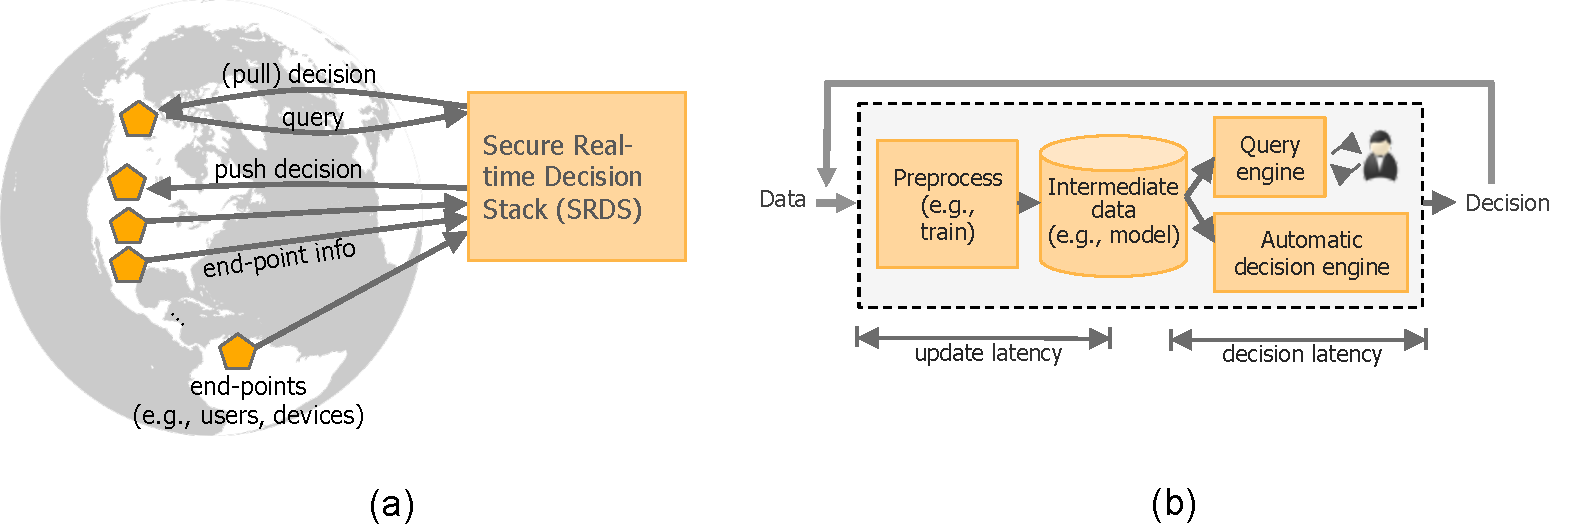
\includegraphics[scale=0.6]{figures/model-and-decision}
}
 \caption{\small{(a) High-level SRDS architecture. (b) Typical decision system.}}
  \label{figure:model-and-decision}
\end{figure}

Figure~\ref{figure:model-and-decision}(b) illustrates a simple decision system. At the high level, decisions are based on the data entering the system. In addition, the decisions can be impacted by the outcomes of the previous decisions. We call these systems ``feedback-based decision systems''.

The decision process consists of two stages. In the first stage, the raw data is transformed into an intermediate representation. A classic example of an intermediate representation is a model trained on the raw data. The second stage is where the decision actually happens. There are two types of decisions: manual and automated. With manual decisions, there is a human in the loop that queries the intermediate state (e.g., model) to make decisions, while with automated decisions there is no human in the loop.

There are two metrics that characterize the decision system performance: update latency and decision latency. The update latency determines how fast are the changes in the input data reflected in the intermediate data. The update latency determines the freshness of the model, and it is critical in a dynamic system where the model changes over time. Consider a scenario as simple as clustering tweets based on the location they originate from. As the set of active users changes, the centers of the clusters shift. As a result, the update latency can have a significant impact on the accuracy of the clustering algorithm. The decision or query latency represents the time it takes to query the intermediate data (e.g., model) in the case of human decisions, or the time it takes to make a decision in the case of automated decisions.


The space of making decisions on (big) data is a huge one. Next, we summarize what is and what is not in the scope of this proposal.

{\bf Backend vs. Endpoint Decisions:} Today, several high-profile real-time decision systems are implemented at the endpoints (e.g., self-driving cars, autonomous robots). While endpoints will remain instrumental in the decision making process, and in some cases will be the critical components of a decision system, our vision is that, going forward, more and more of the decision logic will migrate to the backend. There are several reasons for this. First, a backend engine can make decisions on the global information shared by multiple endpoints. Learning from the collective feedback of multiple endpoints can lead to better decisions than locally learning from a single endpoint. Second, a backend is much easier to scale and in general has to a much larger pool of resources than a single endpoint, which means that it can implement far more sophisticated algorithms. Finally, it is typically much easier to deploy and update software on a backend system than on endpoints. This will enable a much faster evolution of the algorithms and tools.

Of course, this will not obviate the need for endpoint-based decisions systems, or endpoints taking an active part in the decision process. Endpoints will still be the best place to implement decision algorithms for cases that require super-low latencies (e.g., self-driving cars), or that require processing huge amounts of data, such as video. However, even in those case we believe that some of the functionality will migrate to the backend or additional functionality will be deployed in the backend to augment the endpoint decisions. Examples of endpoint decision systems that will be augmented by a backend decision engine are self-driving cars sharing the information to improve driving algorithms (i.e., fleet driving), and coordinating a fleet of drones sharing the same airspace.  

For these reasons, in this proposal we will be primarily focusing on building and developing backend decision systems, such as SRDS, rather than endpoint decision systems, such as self-driving cars. This being said, we do plan to work closely with other groups at UC Berkeley and elsewhere that focus on developing endpoint decision systems, work with the community to standardize the APIs between endpoints and backend, as well as build prototypes of endpoint decision systems whenever possible.  

%{\bf Decisions vs. Actions vs. Hints:} We are using words ``decision'', ``action'', and ``hint'' interchangeably. In particular, ``decision'' also covers the case in which SRDS instructs an endpoint to take a particular action (e.g., changing the driving direction of an autonomous car), and the case in which it provides hints which the endpoint may choose to ignore (e.g., let a driver know about a better available route).    

{\bf Scope of Applicability:} We have chosen to focus on supporting secure, real-time decisions on live data, as it is our belief this is the next big challenge in big data processing, and has the ability to fundamentally change the way we build intelligent systems. That being said, we expect the techniques we develop in this work to have a much broader, and even more immediate, applicability, by handling other use cases, such as decisions on historical data, high throughput interactive query workloads, low latency streaming, and secure big data processing.

At the same time, our intention is not to build a replacement for existing highly successful systems that already perform real-time decisions on live data, such as high-frequency trading and real-time ad bidding. These systems are highly-optimized for the task at hand, and, in many cases, took many years and billion dollars to build. Instead, our goal is to dramatically lower the cost and time to develop the next wave of such applications. This is similar to the way Hadoop and Spark did not target the specialized systems to index the web back in the days, but focused on democratizing big data processing, by enabling virtually everyone to build big data applications.


\section{Research Challenges }

In this section, we discuss the research challenges we plan to tackle as part of this proposal.


\subsection{Real-time Decisions on Live Data} 

Despite existing examples such high-frequency trading and real-time ad targeting, making real-time decisions on live data is hard. This difficulty is because these decisions need to simultaneously achieve high quality, low latency, and be secure. Next, we define and discuss each of these desirable attributes.

{\bf Quality}: By quality we mean the ability to make complex decisions that are accurate and robust. Many decisions are non-trivial. For example, detecting attacks in the Internet, coordinating a fleet of flying drones, or fraud detection, involve all complex decisions. Furthermore, many of these decisions should be automated. Without humans in the loop, we need to make sure that these decisions are both accurate and robust. 

By accuracy, we mean the ability to minimize both false positives and negatives. The failure to do so may lead to undesirable outcomes. For example, in the case of a fraud detection system, not catching a fraudulent transaction or blocking a legitimate transaction can both lead to revenue loss for a credit card company~\cite{Sculley11}. 

Furthermore, decisions should be robust in the presence of noisy data or unforeseen inputs. For example, a system coordinating a fleet of drones will have to deal with the noisy inputs provided by the sensors of the drones (e.g., a blurry video feed during heavy rain). As another example, consider an application that aims to detect Internet attacks (e.g., viruses, worms). Since these attacks are continuously evolving, such an application will have to deal with unforeseen attacks.

{\bf Latency}:  Ideally, one would like to minimize both the update and the decision/query latencies. However, there is a trade-off between these latencies.  In general, the more of the decision process we materialize in advance the faster the decision. Indeed, in settings where the space of decisions is finite one can precompute all possible decisions. This option will minimize the decision latency at the cost of the update latency.  At the other extreme, one can directly query the (raw) input data. In this case, the update latency is zero, but the decision latency will be much higher.  In~\cite{Crankshaw15} we began to explore this tradeoff in greater detail and identifying mechanisms to dynamically trade-off these two latencies.

{\bf Security}: To make increasingly better decisions, users and organizations amass even more data, leading to  disastrous confidentiality and privacy breaches when compromised. Hence, as the amount of data grows, the need for security and the impact of the lack of security expands as well. Security attacks have already reached vast amounts of private or confidential data~\cite{breaches2015}. For example, last year marked the largest theft of medical records to date when attackers stole tens of millions of medical records from two major health insurers, Anthem and Premera~\cite{AnthemBreach,AnthemLargest}. 
%It is estimated that attackers stole records of 80 million people from Anthem, and records of 11 million people from Premera. 
The data stolen included names, SSNs, medical information, and financial information. Furthermore, governments everywhere are pushing for back-doors into public services and subpoena companies providing those services to access user information in the name of security. 

Security breaches and personal information leakages can undermine the trust of the users in a service or application. This mistrust might lead to the demise of a service, as it may cause user defection, or worse it may expose the service owner to costly litigations. On the flip side, strong privacy guarantees may attract more users, which will ultimately lead to better decisions and better services. 
%Security can also provide a competitive advantage to a service.

In addition, more of these applications and services are being deployed in public clouds, such as Amazon Web Services, Microsoft Azure, or Google CE. As such, providing both data and computation integrity are critical to protect and secure these services against concerns regarding malicious employees of cloud providers, or tenants that share the same cloud infrastructure. While ensuring these security properties is difficult, the real challenge is doing so while preserving the functionality and the performance of these applications.

\subsection{General Purpose Solution}

Virtually all state-of-the-art systems~\cite{Agarwal14, Graepel10, Ganjam15}  we have discussed so far are custom, they have taken a long time to build, and their development was expensive, in some cases costing billion of dollars. Such is the case for search engines, navigation systems, self-driving cars, voice personal assistants, high-frequency trading, and ad targeting. To the extent there exists general platforms in this space, such as Spark or Hadoop, they only provide a solution to part of the problem. They do not  provide an end-to-end secure real-time decision stack. Looking forward, we believe there is the potential for an explosion of applications incorporating real-time decision making on live data. However, if this potential is to be realized, we would need to make it much easier to build and maintain such applications. 

\subsection{Why Now?}

While supporting secure real-time decisions on live data raises daunting challenges, we believe the time is ripe for addressing them, and we are in a unique position to do so. Recent hardware trends will enable the design of a new generation of cluster computing frameworks with dramatically higher performance and stronger security than the existing solutions: 

\begin{itemize}[noitemsep,topsep=0pt,parsep=0pt,partopsep=0pt]
\item The proliferation of hardware enclaves, which are now part of both Intel and ARM chips, enable one to securely run arbitrary code on an untrusted computer system.

\item The emergence of new architectures that tightly integrate CPU and FPGA/GPU. For example, the latest Intel Xeon processor integrates CPU and FPGA on the same chip, and numerous vendors are working on systems in which  CPUs and GPUs share the memory via a High Bandwidth Memory bus.  

\item With the advent of RISC V, the first open instruction set architecture, it is easier than ever to build custom chips that optimize performance for various workloads and integrate new security features.

\item The emergence of the next generation of fast persistent storage systems. Just a few months ago, Intel and Micron have announced 3D Xpoint, a storage technology that can achieve the density of SSDs while providing latencies close to those of DRAM. Systems based on these new technologies will be released later this year, and have the potential to revolutionize the way we built data processing systems.
\end{itemize}



\section{Application Examples}

In this section, we discuss several examples of potential applications that will be enabled by the ability to make secure, real-time decisions on live data. We characterize these applications by using the three decision attributes described in the previous section: decision quality (which captures the ability to make complex, accurate, and robust decisions), decision latency, and security.

Table \ref{table:apps} shows the characteristics of ten such applications. These applications have a broad set of requirements across various attributes. Next, we describe three of these applications examples in detail.

\begin{table}[h]
\begin{center}
{\small
\begin{tabular}{ |c|c|c|c|c| } 
 \hline
{\bf Applications} & {\bf Quality} & \multicolumn{2} {|c|}{\bf Latency} & {\bf Security} \\\cline{3-4}
& & {\bf Decision} & {\bf Update} & \\\hline 
Zero-time defense & complex, accurate, robust & sec & sec & privacy, integrity \\\hline
Parking assistant & complex, robust & sec & sec & privacy \\\hline
Disease discovery & complex, acurate & min & hours & privacy, integrity \\\hline
IoT (smart buildings) & complex, robust & sec & min/hours & privacy, integrity \\\hline
Earthquake warning & complex, accurate, robust & ms & min & integrity \\\hline
Manufacturing pipeline & complex, accurate, robust & sec/min & min & confidentiality, privacy \\\hline
Fraud detection & complex, accurate & ms & min & privacy, integrity \\\hline
``Fleet'' driving & complex, accurate, robust & sec & sec & privacy, integrity \\\hline
Virtual companion & complex, robust & sec & min/hour & integrity \\\hline
Video QoS & complex & ms/sec & min & privacy, integrity \\\hline
\end{tabular}
}
\end{center}
\vskip -0.15in
\caption{\small{Example of applications that would be enabled by a platform for secure, real-time decisions on live data.}}
\label{table:apps}
\end{table}

\subsection{Zero-time defense}

A worm can infect millions of machines in seconds (e.g., at the peak, the SQL Slammer worm was scanning more than 55 million IP addresses per second~\cite{SQLSlammer}). A possible solution to address this problem would monitor the traffic of hosts and users in the Internet, detect worms in real time, and defend from these attacks by patching the software or installing rules at firewalls in real time. While there have been similar proposals in the past, none of them has been widely deployed. We believe that their failure is due to their lack of one or more of the following three properties:

\begin{itemize}[noitemsep,topsep=0pt,parsep=0pt,partopsep=0pt]
\item {\bf Quality}: Decisions need to be robust and accurate. A system with high false positives or negatives would be unusable, as it would either fail to detect attacks, or impair legitimate services by wrongly classifying them as attacks.
\item {\bf Latency}: Not only the decision latency but also the update latency should ideally be in the sub-second range. Indeed, each virus has a slightly different signature so one needs to quickly derive and update the model. 
\item {\bf Security}: Strong security is key. In particular, without strong privacy users and organizations would not allow their traffic to be monitored, and without providing data and computation integrity, these algorithms would be susceptible themselves to attacks.
\end{itemize}

\subsection{Intelligent Parking Assistant}

In many congested downtowns or during sport or concert events it is notoriously hard to find parking spots. This application will alleviate this problem by using a fleet of drones as well as other video feeds to detect available street parking in real time and direct the cars to the available slots via a mobile application. 

Such an application will need to coordinate the drones to efficiently search for parking spots in an area, make sure that the parking spots are indeed available (e.g., there are no signs that precludes parking), identify the type of parking space (e.g., handicap, time limited, payed), and then coordinate cars so that each of them is directed to the closest parking spot available that satisfies the driver constraints (e.g., time duration, non-handicap parking). Of course, the application should also avoid sending multiple cars to the same parking spot. Thus, such an application should has the following requirements~\cite{Quaritsch08, Mottola14}::

\begin{itemize}[noitemsep,topsep=0pt,parsep=0pt,partopsep=0pt]
\item {\bf Quality}: Decisions are complex and need to be robust. In particular, one needs to correctly identify the parking spots that are indeed available in a variety of lighting conditions, signs that might be hidden by vegetation, and imperfect real-life conditions, such as cars being illegally parked.
\item {\bf Latency}: The model capturing the parking spot availability must be updated at second level granularity as parking spots become (un)available or traffic is re-routed, which often happens during events. Decisions should happen at similar granularity as they need to reflect these changes.
\item {\bf Security}: Providing privacy is a big concern, as we want to avoid the risk of turning this application into a surveillance system.
\end{itemize}

\subsection{Infectious Disease Discovery}

Over the past few years we have witnessed the emergence of several aggressive infectious diseases, such as Ebola and Zika, that have claimed lives, spread quickly, and have been difficult to contain. 

Now, imagine  we have the ability to test cheaply a person for a given infectious diseases in minutes, or even seconds. That would fortify our ability to defend against these diseases, as it would allow us to perform effective quarantine at borders (e.g., everyone who is flying in from an infected region can be tested in minutes or seconds before entering the country) and monitor the spread of the disease in real-time, which is especially important for airborne diseases.

The emergence of mobile testing devices such as Nanopore's MinION~\cite{minion} is a step towards achieving this vision. MinION can analyze DNA, RNA, proteins, or small molecules in hours at a cost of several hundred dollars per test. Weighing less than 100g, MinION can be connected to any computer, which makes it a truly portable testing station. Some of us are already working with Dr. Charles Chiu from UC of San Francisco to develop tests to identify Zika virus using Nanopore's MinION . 

Given the expected improvements in the analysis times and test costs reductions over the next couple of years, this research would enable a wealth of new applications that can provide effective tracking of the diseases in real-time, infectious disease risk assessments, as well as accurate and quick testing. These applications will share the following characteristics:

\begin{itemize}[noitemsep,topsep=0pt,parsep=0pt,partopsep=0pt]
\item {\bf Quality}: Decisions need to be robust as they often deal with noisy samples. Inaccurate testing results could have serious implications on the people who are tested, and may lead to suboptimal quarantine decisions.  
\item {\bf Latency}: Models of how a disease spreads, or of the infection risks of the inhabitants in a given area, or of the risk that certain incoming visitors are infected should be updated hourly or faster. Decisions of whether to test a particular person, or whether the test was positive or negative should ideally happen on the order of minutes, even seconds.
\item{\bf Security}: Maintaining the privacy and confidentiality of the results is critical for both the people who are tested and for the population in general. Leaking information, especially inaccurate information, could cause widespread fears.
\end{itemize}


\section{Existing General Purpose Platforms} 

Today's general purpose data platforms fall short of supporting secure, real-time decisions on live data. To illustrate this point, consider a movie recommendation engine as shown in Figure~\ref{fig:related}. Users logs (e.g., viewing preference, ratings) are collected via a message broker such as Kafka and stored in a distributed files system, such as HDFS or S3. A Hadoop or Spark job will periodically read these logs and train a model to capture user recommendations. Then, these models are pushed into a key value store, such as HBase or DynamoDB, from which they are served to users. For instance, when a user logs in, the application will query the key-value store to retrieve the movie recommendations for that user. While such a key-value store can provide millisecond-level delays, this solution has several significant drawbacks:

\0
\begin{figure}[h]
  \center{
 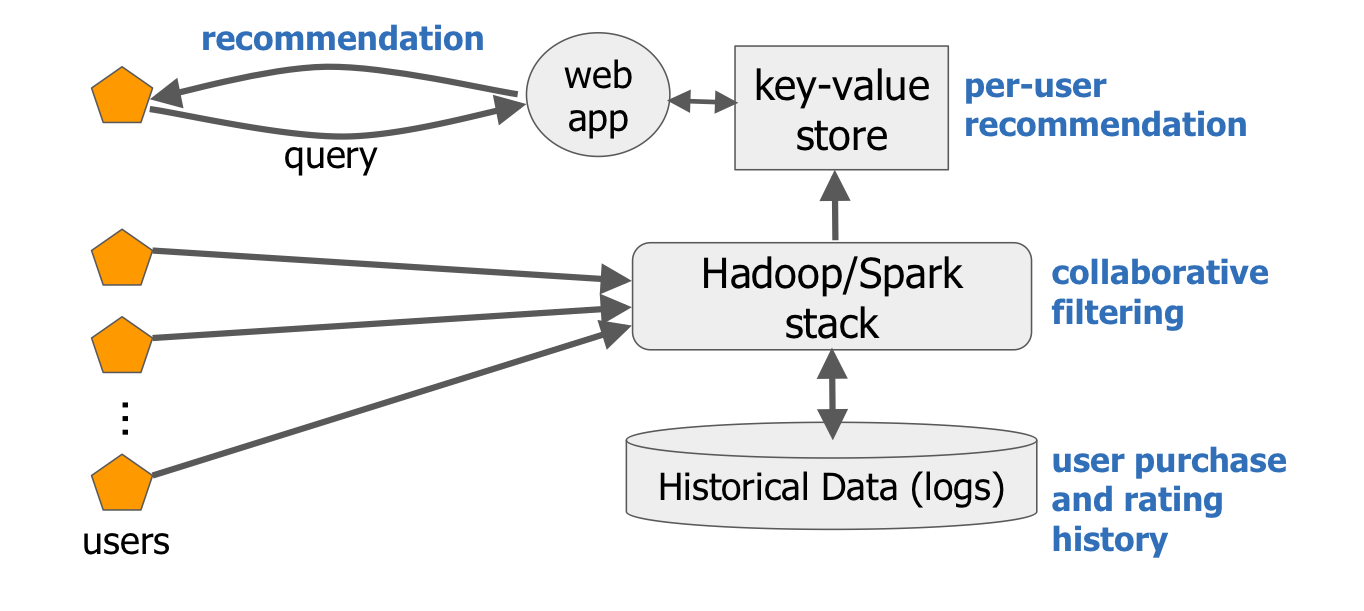
\includegraphics[scale=0.35]{figures/existing-solutions}
  }
  \vskip -.15in
  \caption{\small{The implementation of a recommendation system.}}
\label{fig:related}
\end{figure}



{\bf Simple decisions}: With a simple key-value store it is hard to support sophisticated decisions, such as ML classification or clustering. One way to support such decisions would be to pre-compute all possible decisions. Unfortunately, in general, this is infeasible due to ``the curse of dimensionality''~\cite{Agarwal14, Crankshaw15}. Another possibility would be to run non-trivial algorithms on non-trivial amounts of data. Unfortunately, this will compromise the query latency.  

{\bf Slow updates}: Typically, the intermediate representation (e.g., model) is updated hourly, or even daily. While Spark increases the update frequency it is still in the order of hours, as one needs to read data from the distributed file system, re-compute the model and push the changes to the key-value store.

{\bf Weak security}: In most existing solutions, the main security measure employed is encryption at rest or encryption over the network. The pre-processing and decision logic run with access to decrypted data and are thus vulnerable to any 3rd party attacks or to insider attacks. This is in particular troublesome when computations run on the public clouds, which is fast becoming the norm, rather than the exception. 

In the research community, two techniques are emerging as possible solutions to protect the application's integrity and user's privacy. The first is computing on encrypted data which was first proposed in the theory community~\cite{databanks78, gentry2009fully}, and then popularized in practical systems by CryptDB~\cite{cryptdb} and Mylar~\cite{mylar}. The second is leveraging hardware enclaves~\cite{IntelSGX}, which are now integrated in both Intel and ARM chips to securely run arbitrary software in untrusted environments, such as the public cloud. However, none of these techniques are perfect. While computing on encrypted data makes minimal assumptions about the hosted environment, it can support only a limited functionality on encrypted data. In contrast, hardware enclaves allow one to run arbitrary code, but they leak data if there are bugs in the trusted code running in the enclave, if untrusted code runs in the enclave, and from various side channels~\cite{SGXmemorychannel, SGXnetworkchannel}.



\section{Proposed Research}
\label{sec:research}

Table~\ref{table:new-work} summarizes the state-of-the-art of the decision systems today. On one hand, there are few successful systems that perform real-time decisions on live data, and those that do are special-purpose and very expensive to develop. On the other hand, the existing general purpose stacks fall short of providing support for such decisions, and they have weak security. Next, we discuss the proposed work to provide platform, tools, and algorithms to support general purpose secure, real-time decisions on live data.  


\begin{table}[h]
\begin{center}
{\small
\begin{tabular}{ |c|c|c|c|c| } 
 \hline
{\bf System} & {\bf Quality} & {\bf Latency} & {\bf Security} & {\bf General Purpose}\\\hline 
High Frequency Trading & High & Low & High & No \\
Ad Targeting \& Bidding & & & & \\\hline
Hadoop, Spark & Average & Average & Weak & Yes\\
                         &               & (slow updates) & & \\\hline
{\bf Proposed Work} & {\bf High} & {\bf Low} & {\bf High} & {\bf Yes} \\\hline
\end{tabular}
}
\end{center}
\vskip -0.15in
\caption{\small{Comparison between state-of-the art decisions systems/stacks and proposed work.}}
\label{table:new-work}
\end{table}


\subsection{Systems}

To meet the performance and the functionality targets we need to build a new software stack. That software stack should at a minimum, in similarity with our prior work on the Berkeley Data Analytics Stack (BDAS), enable developers to write sophisticated applications, including deep learning and model serving. Such a stack should achieve the following properties when compared to previous stacks such as BDAS, Spark~\cite{spark}, and Hadoop~\cite{murthy2011architecture}:

\begin{itemize}[noitemsep,topsep=0pt,parsep=0pt,partopsep=0pt]
\item Provide similar functionality to Spark, i.e., enable developers to write sophisticated applications, including ML and graph processing applications.
\item Achieve 100x lower query latency, and 1,000x higher throughput.
\item Provide fine-grain reads and writes to better support new applications such as deep learning and model serving (which are poorly supported by general purpose big data stacks, such as Spark).
\end{itemize}

To satisfy these requirements, we plan to build a highly modular architecture around a kernel that will provide very high performance scheduling and resource management. This approach is akin building a {\em microkernel} for big data processing frameworks. This will require us to re-architect today's monolithic data computation engines, such as Spark. This includes parallelizing the control plane, supporting new computation models, besides the traditional Bulk Synchronous Protocol (BSP) model, and providing support for fine-grain updates. Increasing concurrency for both computation and access to storage while preserving the fault tolerance properties of existing cluster computing frameworks will require new techniques and algorithms. 

In addition, we intend to build an abstraction that combines the best of today's big data storage abstractions, such as HDFS, pub-sub systems, such as Kafka, and NoSQL serving layers, such as Cassandra. This would obviate today's need for transferring data between different storage layers. The system would be optimized to be able to handle read-heavy workloads, which existing systems such as HBase~\cite{hbase} are poor at (due to structures such as LSM-trees). The system should be pluggable so that advanced logic can be added on top of the serving layer, enabling advanced machine learning predictions. 

\subsection{Security} 

Our goal is to provide privacy, confidentiality, and integrity without impacting performance or functionality. The hope is to enable service providers to continue extracting value out of data unhampered, while protecting the data and the computation. This goal is challenging to achieve. Attackers have become very skilled, and traditional security approaches no longer suffice. These approaches assume that a part of the software stack (e.g., the operating system, the language runtime) is trusted and bug-free, and ensures that a higher-level application cannot be attacked. Attackers have managed to bypass such techniques by, for example, obtaining root access on machines.

We aim to build a security platform that preserves the privacy and integrity of data at a service provider against any software attacks. Even if an attacker obtains root access on the server machines, the attacker cannot extract the data or modify the data or the computation on the data. This strong security guarantee automatically addresses a large class of attackers.

Providing such strong security guarantees not only helps organizations preserve the data value and protect their reputation, but likely, it can increase this value. More users or organizations will likely want to participate in a certain service if they have the guarantee that their data will remain private or confidential, and they can trust the interaction with this service.
                                               
To provide such strong security we are planning to leverage the recent advances in hardware and secure algorithm design. On one hand, new Intel and ARM chips have started to include hardware enclaves~\cite{IntelSGX} which allow one to securely run arbitrary code that is fully protected against malicious applications, and even against a malicious operating system.  On the other hand, advancements in performing computation on encrypted data allow us to provide privacy and confidentiality to non-trivial applications, such as databases and web applications, without hardware support. 
We plan to build new systems that combine the strengths of hardware enclaves and computation  on encrypted data while obviating their weaknesses, i.e., systems that provide strong security without impacting the decision's latency or quality. This requires work at the level of designing new systems, security protocols, cryptographic schemes as well as at hardware design. The current hardware enclave proposals, while being a significant first step, suffer from both complexity and security issues~\cite{SGXcostandevadas}. We plan to design a clean and secure hardware enclave based on RISC-V, which provides a flexible, open infrastructure to perform this research. 
%We hope that our design will inform industry deployments. 


\subsection{Machine Learning} 

Automated decisions required by applications such as zero-time defense, agile robotic systems, and distributed sensor networks provide tremendous opportunities for machine learning. As the role of machine learning expands to these ambitious applications, however, it is critical these new technologies be safe and reliable.  Failure of such systems could have severe social and economic consequences including the potential loss of human life. How can we guarantee that our new data-driven automated systems are robust?

Despite tremendous success in recent years, machine learning remains a delicate technology. It can take dozens of experts to train, calibrate, and maintain a single machine learning pipeline. More troubling, in both scientific and industrial applications, it is never clear how a machine learning system will truly perform on unseen data until the model goes live in a mission critical environment. In order to make machine learning more robust, several important questions must be addressed:

{\bf Robust methods for optimization:}  (Note this is in stark contrast to robust optimization, which is about modeling, not about methods).    While the theoretical study of optimization has largely focused on ``faster is better'' (along with the precise characterization of rates of convergence), it is often the case that practical considerations (including noise tolerance, parallelizability and communication constraints, asynchronous updating) make such improvements moot (e.g. the theoretically fastest methods such as ``acceleration'' are brittle in practice, for a variety of reasons). Can we provide scalable optimization procedures, which are provably accurate when taking into account modern considerations such as noise tolerance and parallelization with realistic communication models? Furthermore, can we also provide better procedures for non-convex optimization, both provably and in practice? Non-convex optimization procedures are widely used in deep learning, and effective parallel algorithms remain elusive for these methods.

{\bf Modeling uncertainty:} In order to make reliable real-time decisions, we must understand how a machine learning system will perform when it is released in the wild.  It is critical that the models are designed to be robust to perturbations that are not in the training data.  In controls, this sort of uncertainty is managed at design time: a worst-case uncertainty is place in the loop with the controller and the controller is optimized to reject these unknown disturbances.  For machine learning rather than such worst-case approaches, we lean on randomness and hope the unseen data is identically distributed to that in our laboratory.  Adapting the techniques from robust control, is it possible to train machine-learning systems to perform at a high level, yet be robust to unforeseen aberrations in the real world data?  How can we model such uncertainty to not overly reduce performance?  And can we design adaptivity into our learning systems so that they can correct for changes in data distributions after they have been released?

{\bf Data-driven Dynamics:}  What is the appropriate granularity to incorporate fresh data into machine learning models?  In order to incorporate this fresh data, we must understand how time-varying models affect performance and reliability.  In machine learning, dynamics are typically integrated into models as an afterthought, not in a principled way.  For example, in recurrent neural networks, dynamical systems are unrolled and treated as feed-forward models.  Furthermore, as models interact with the world they affect the data they see in the future reinforcing biases in a closed feedback cycle~\cite{Li10, Bottou13}.  The fundamental notions of feedback, stability, and sensitivity are not considered.  On the other hand, tools from dynamical systems rely on well-prescribed differential/difference equations models.  Our understanding of how to identify non-parametric, nonlinear dynamical systems is limited.  How can we bridge the gap between the statistical tools of machine learning with the dynamics-centered techniques from control theory?


\section{Knowledge Transfer and Prototype Systems}

{\bf Knowledge Transfer:} Over the years, the systems group at Berkeley has had great success transferring their technology by distributing open-source software (\eg BSD and Postgres) and engaging with companies to promote radical new technologies (e.g., RAID and RISC).  More recently, the AMP and ASPIRE labs have transferred a wide range of technologies, including Apache Mesos, Apache Spark, and RISC V. Apache Spark is the most popular big data framework today, with over 1,000 contributors, over 60,000 meetup members world wide. IBM has called it ``the Most Significant Open Source Project of the Next Decade'' and ``the OS of the Big Data'', and last year announced a \$300 million investment to develop Spark. Spark is included in virtually every big data software distribution, and is used by thousands of organizations in productions. Apache Mesos is the first operating system for datacenter, and now in used at major companies to manage thousand-node datacenters, including Twitter, Apple, and GE.  Furthermore, RISC V, the first open source instruction set architecture that is already disrupting the CPU and custom ASIC markets. Google, HP Labs, and Oracle, just to name a few, are members of the RISC V foundation, and many companies have already started to develop chips based on RISC V. Finally, Berekley students and faculty have founded companies to support these open source efforts for all these projects.

This project will continue this tradition, by developing a suite of software tools and algorithms which will dramatically lower the barrier for organizations and indiviudals alike to build decision and predictive analytics applications. We hope this platform will have a significant impact in the industry, and will lead to the creation of new companies and the development of new applications which were not possible before.

%\cite{late-osdi,delay-scheduling-eurosys,mesos-hotcloud,mesos-techreport,drf-techreport,spark-hotcloud,perf-prediction-icde,scads-cidr,piql-socc,replay-sosp,log-mining-sosp,online-log-mining-icdm,fingerprinting-eurosys,spikes-socc,xtrace-nsdi,ml-security-sigmetrics,ml-security-leet,policy-aware-sigcomm,ml-security-raid,stat-debugging-icml,ethane,of-ccr,nox}

{\bf Industry Participation:} As with the AMP  Labs (which had over 30 industrial partners over its five years), industrial participation in the new project will be crucial to its success.  Only through close and constant interactions with industry can we learn about the problems that arise in large production systems.  We are at the early stages to involve the industry on this project, but the early sings are very promissing. We expect that starting with 2017 to raise \$1M-\$1.5 dditional per year from these partners. While this funding certainly provides additional resources, it is perhaps even more useful in cementing the level of commitment our industrial partners have to a long-term collaborative relationship.

\section{Outreach}

Like with AMP Lab, we will inspire students under-represented groups to pursue rewarding careers in computer and information science and engineering through the following steps:

{\bf Leading by Example:} Of the XXX members of the  team, two are women, and two are belong to under-representative minorities.  While we cannot predict which students will work on the next project, we note that out of the 50 postdocs and students currently sitting in the AMP Lab (excluding those belonging to a faculty member not participating in this effort) XXX are women and one is a under-represented minority.  Moreover, the PIs have been leading the EECS departmental efforts (chairing the diversity committee and the recruiting committee) that recently led to the hiring of three women faculty over the past two years (one of them, Raluca Popa, is participating this project as a co-PI).

{\bf Boardening Training and Academic Impact:} over the past few years, we have trained over 40K students on Spark and thousands on Mesos and Tachyon. We have done this via annual boot camps, running training classes at big data conferences, such as Strata, Hadoop Summit, and Spark Summit, and MOOCs.  Right now Apache Spark is used at tens of universities across the globe in data science classes. AMP lab has also produced leaders in their fields both in academia and  industry. The AMP lab alone has produced students who are now faculty members at top universities, including MIT (3 faculty members), Stanford University (3 faculty members), UIUC, and University of Michigan. In addition, Matei Zaharia won the ACM Best Dissertation Award and John Duchi an Honorable Mention for the ACM Best Dissertation Award, both in 2014. Similarly, several students have gone to found companies to support the open source software we developed, including Databricks, Mesosphere, and Alluxio. 

{\bf Leveraging  Local Programs:} This project will leverage the ongoing campus diversity programs, BFOIT and SUPERB. The Berkeley Foundation for Opportunities in Information Technology (BFOIT) \cite{bfoit} supports historically underrepresented ethnic minorities and women in their desire to become leaders in the fields of computer science, engineering and information technology. 
%The intent is to provide youth with knowledge, resources, practical programming skills and guidance in their pursuit of higher education and production of technology.  
Berkeley's College of Engineering has been a leader in offering opportunities to underrepresented undergraduates to work on research projects through the Summer Undergraduate Program in Engineering Research at Berkeley (SUPERB) Program \cite{superb}.  

{\bf Broadening Research Participation:} The SRDS system will put a set of sophisticated data processing tools in the hands of all interested researchers.  Researchers will be able to use SRDS directly to explore new applications, or contribute their own algorithmic modifications.  In addition, for researchers that cannot afford to pay for cloud-based computational services, we will make our own computational resources available for them to run SRDS. We have already done this in the case of Spark. One of the startups we founded, Databricks, is now providing a free hosted version that allows everyone to learn Spark.

{\bf Broadening the Information Economy:} If our project is successful, it will increase human participation in data analysis.  This will provide employment opportunities for any individual with Internet access.  And more than just providing a job, this will provide entry-level positions in the information economy that do not require extensive training, but yet hold the potential for more expansive roles as they gain experience and expertise.  

\section{Management and Collaboration}

Creating an effective collaborative climate among an interdisciplinary team of researchers is a daunting task. However, for the past five years most of the team has worked together closely over the past five years as part of Berkeley's AMP and ASPIRE labs.  These brought a diverse group of researchers (with expertise ranging from machine learning to networking to operating systems to security to computer architecture) together to explore the new field of datacenter computation. Almost all publications from the AMP Lab involved interdisciplinary teams, with strong input from industry experts.

The AMP and ASPIRE Labs used a variety of measures to facilitate collaboration, and we expect to leverage these same practices for this project.   To foster collaboration, we will have:

\begin{itemize}[noitemsep,topsep=0pt,parsep=0pt,partopsep=0pt]
\item Weekly all-hands meetings for talks on recent progress and to discuss future plans.
\item  Weekly meetings for each of the smaller projects (we expect roughly a dozen such meetings weekly).
\item  Monthly 3 hour faculty-only meetings over dinner, for in-depth technical discussions and long-term planning.
\item  Biannual three-day retreats, where we present results to outside experts (particularly from industry) and discuss their feedback.
\end{itemize}

In addition, the core members of the team will sit in the space developed for the AMP Lab, where both students and faculty share a large open space.  This facilitates ongoing communication among all members of the project and increases faculty-student interactions.

%The lead investigator of the project is Ion Stoica, and he will be responsible for overseeing the effort.  He will be assisted by Mike Jordan and Joe Hellerstein, who will help Stoics ensure that all areas of the project are moving forward.  They will be assisted by two administrative staff.




\end{outline}

\bibliographystyle{abbrv}
%\bibliographystyle{plain}
\bibliography{rise-preproposal}

\end{document}
